
%...........................................................
%
% Method for significance
%
%...........................................................

\section{Method for significance calculation}
\label{app:method_significance}

The significance for a certain oscillation hypothesis given by the measured data is provided as following.
First the $\Delta \chi^2$ distribution, $f(\Delta \chi^2)$, is obtained by many toy experiments (e.g. $10k$),
then the $\Delta \chi^2_{data}$ value is measured with the data set.
This quantities are shown in \cref{fig:joint_dcp_fc_example}.

First the p-value is calculated as:

\begin{equation}
\text{p-value} = \int_{-\infty}^{\Delta \chi^2_{data}} f(\Delta \chi^2) d(\Delta \chi^2)
\label{eq:pvalue}
\end{equation}

\begin{figure*}[htb]
\center
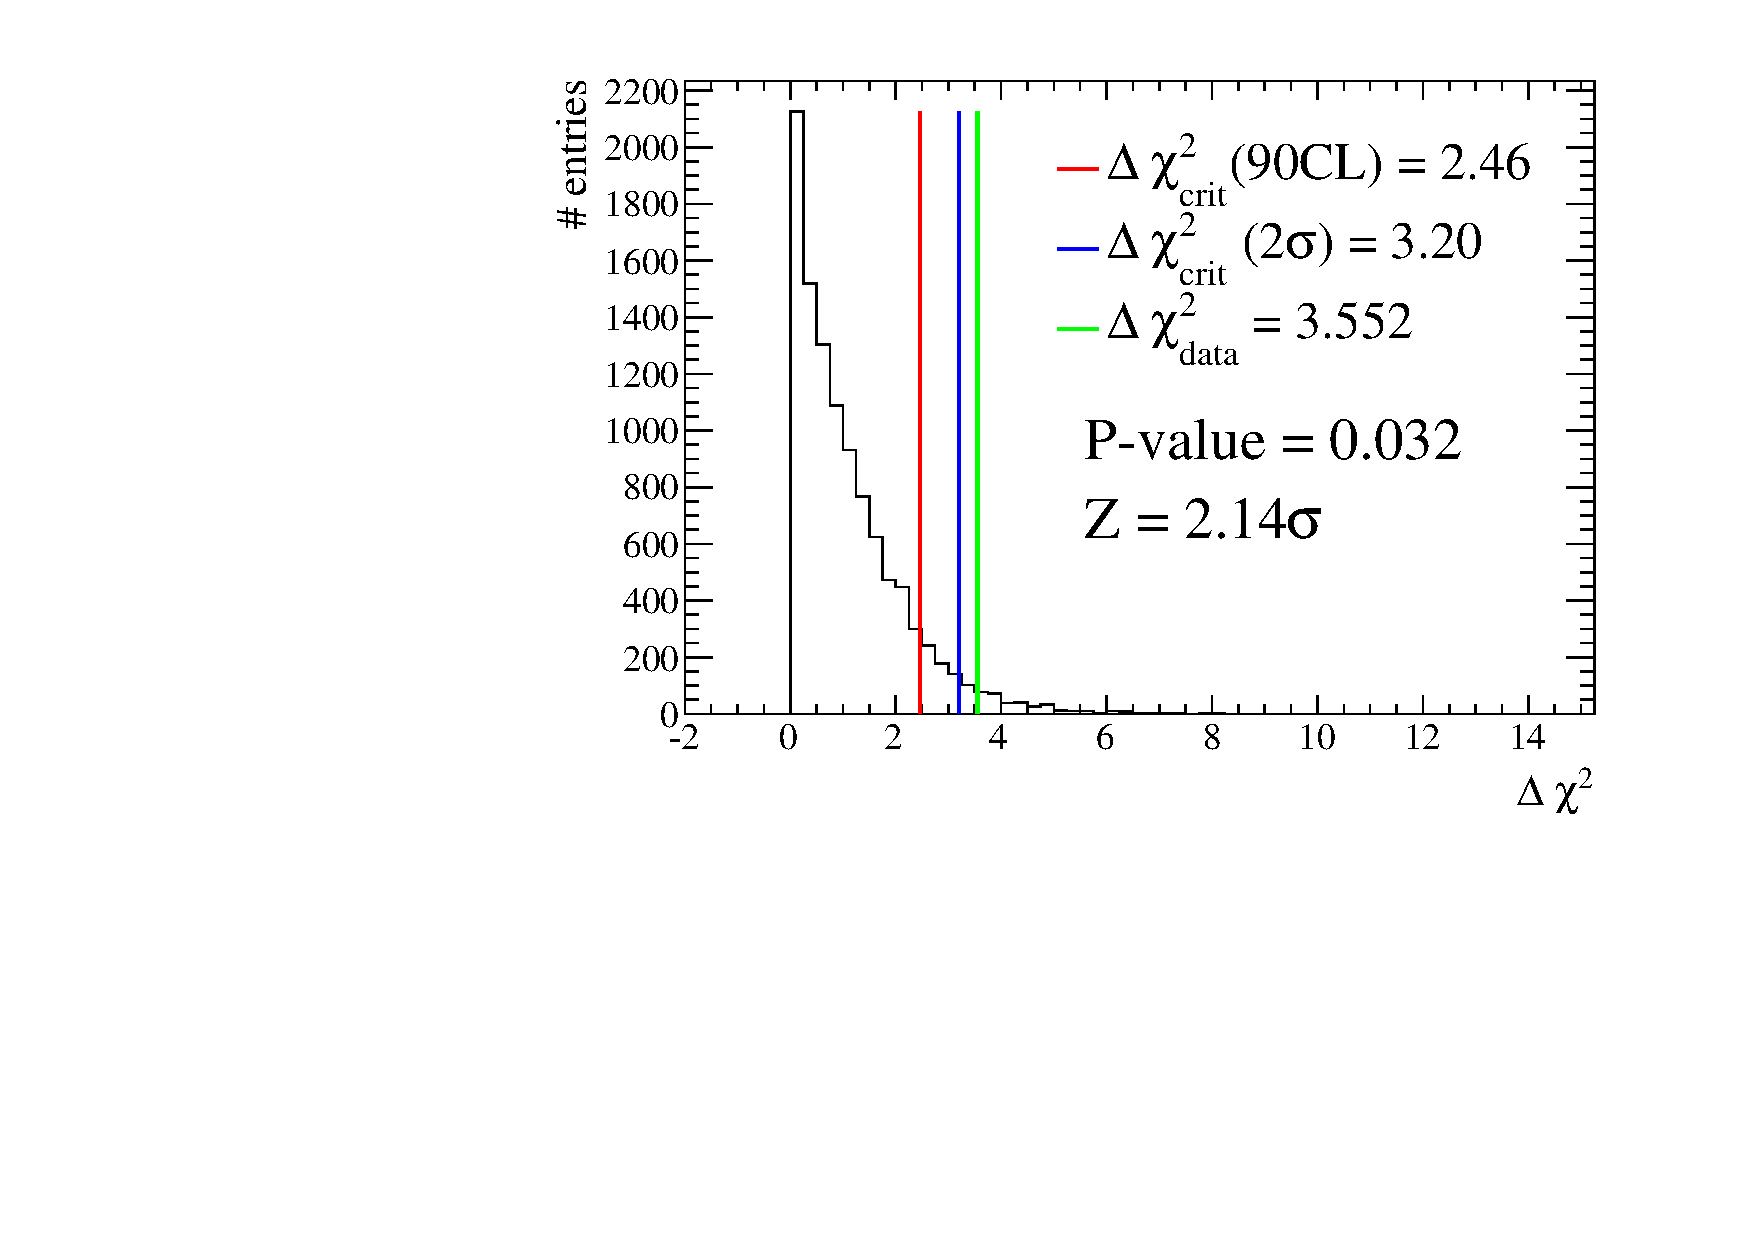
\includegraphics[width=0.49\textwidth]{joint_plots/coverage_fc/fc/significance_nh_dcp_0.pdf} 
\caption{
Distributions of $\Delta \chi^2$.  
$10k$ toy experiments are performed
with true values of $\delta_{CP} = 0$ (left) and $\pi$ (right), 
assuming normal hierarchy and applying the reactor constraint.
Both the mass hierarchy and $\delta_{CP}$ are profiled in the fit.
All the other oscillation parameters are marginalised.
The statistics corresponds to the Run 1-6 data set.
The $\Delta \chi^2$ value (green line) measured from the Run 1-6 data set
as well as the p-value and the significance as number of standard deviations (Z),
are shown as well.
}
\label{fig:joint_dcp_fc_example}
\end{figure*}

Then the significance can be shown as the number of standard deviations
where the measured quantity is assumed to be gaussian distributed.
In \cref{fig:zscore} the gaussian distribution of the measured variable $\mu$ is shown
as a function of the $Z$-score, i.e. how many standard deviations 
a certain measurement $x$ is far from the expected value:

\begin{equation}
Z = \frac{x-\mu}{\sigma}
\label{eq:zscore}
\end{equation}

If an experiment measures $x$,
$\alpha$ is the area of the p.d.f. corresponding to a certain CL (90\% in the example).
The quantity $\sigma$ is the bias of the measured value with respect to the expectation
 that contains $1-\alpha = 68.27\%$ of the total area.

The significance can be reported with the $Z$-score in the following way:

\begin{itemize}

\item the p-value is measured using \cref{eq:pvalue}

\item Assuming the p-value to be 1-sided (see \cref{fig:joint_dcp_fc_example}) and $\alpha$ 2-sided (see \cref{fig:zscore}), 
we set $\alpha = \text{p-value}$

\item $Z$, shown in \cref{eq:zscore}, is computed using the quantile distribution.
	Given the cumulative distribution function of the normal standard distribution with Mean=0 and RMS=1 ($\sigma=1$),
	
	\begin{equation}
	%\Phi(x) = \frac{1}{\sqrt{2\pi}} \int_{-\infty}^x e^{-t^2 / 2} dt, x \in [-x,x]
	%\Phi(x) = \frac{1}{\sqrt{2\pi}} \int_{Z \sigma}^{+\infty} e^{-t^2 / 2} dt = \alpha / 2  
	\Phi(x) = \frac{1}{\sqrt{2\pi}} \int_{Z}^{+\infty} e^{-t^2 / 2} dt = \alpha / 2  
	\label{eq:cumulative_norm}
	\end{equation}
		
%	Then 	
%	\begin{equation}
%	1 - \alpha  = 1 - 2 \Phi(x)
%	\label{eq:cumulative_norm}
%	\end{equation}
	
	the quantile is defined as
	
	\begin{equation}
	%Z = \Phi^{-1} (1 - \text{p-value})
	Z = \Phi^{-1} (1 - \alpha/2).
	\label{eq:quantile_norm}
	\end{equation}
	
	The ROOT function Math::gaussian\_quantile, that takes $\alpha$ as input, 
	and calculate the cumulative distribution function of the lower tail of the normal (Gaussian) distribution
	is defined as following:
	
	\begin{lstlisting}
	TF1 q("q","ROOT::Math::gaussian_quantile(1.-(x/2.)),1.)",0.,1.); 
  	double Zscore = q.Eval(pvalue); 
	\end{lstlisting}
	
\end{itemize} 


\begin{figure*}[htb]
\center
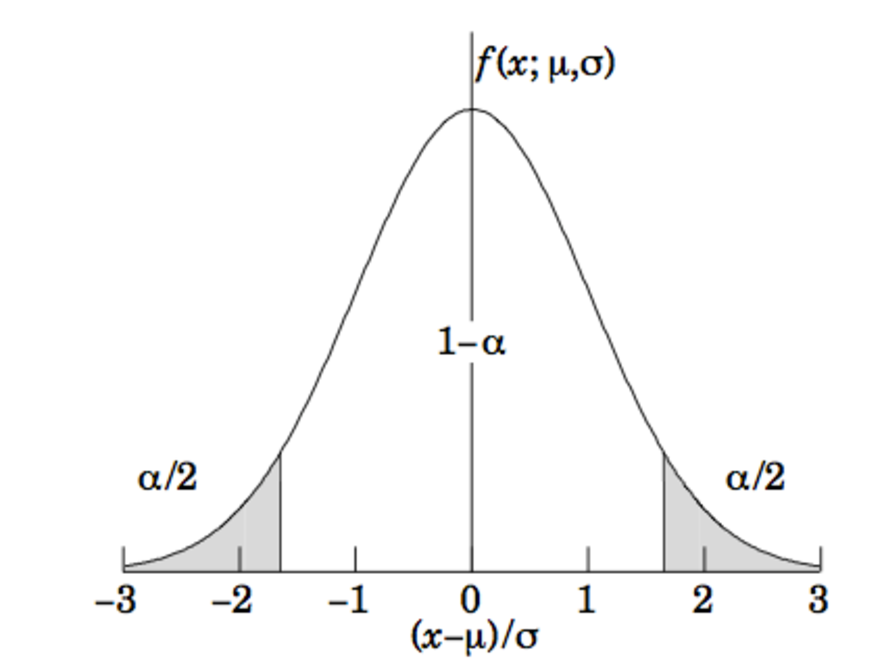
\includegraphics[width=0.49\textwidth]{joint_plots/coverage_fc/Zscore.pdf} 
\caption{
%Representation of  as a function of the Z-score.
 Illustration of a symmetric 90\% confidence interval (unshaded) 
 for a measurement of a single quantity with Gaussian errors. 
 Integrated probabilities, defined by $\alpha = 0.1$, are shown.}
\label{fig:zscore}
\end{figure*}


\clearpage



